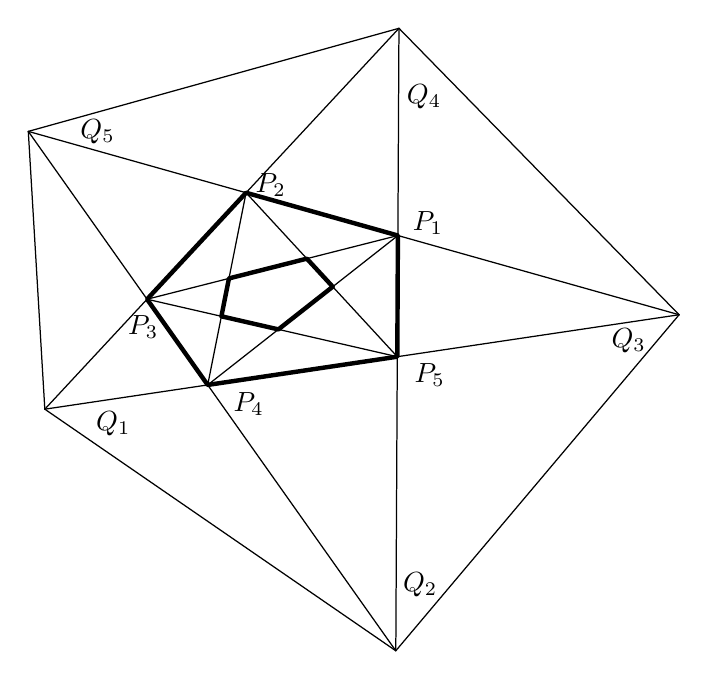
\begin{tikzpicture}[x=.01cm,y=-.01cm,line width=.45pt,line cap=round,line join=round,every node/.style={inner sep=0pt,font=\normalsize}]
\coordinate (Q5) at (392,534);
\coordinate (Q4) at (863,403);
\coordinate (Q3) at (1219,767);
\coordinate (Q2) at (859,1194);
\coordinate (Q1) at (413,887);
\coordinate (P2) at (668.717,611.962);
\coordinate (P1) at (861.668,666.325);
\coordinate (P5) at (860.89,820.317);
\coordinate (P4) at (619.971,856.186);
\coordinate (P3) at (542.909,747.276);
\draw (Q5)--(Q4);
\draw (Q4)--(Q3);
\draw (Q3)--(Q2);
\draw (Q2)--(Q1);
\draw (Q1)--(Q5);
\draw (Q5)--(Q3);
\draw (Q3)--(Q1);
\draw (Q1)--(Q4);
\draw (Q4)--(Q2);
\draw (Q2)--(Q5);
\draw (P2)--(P5);
\draw (P5)--(P3);
\draw (P3)--(P1);
\draw (P1)--(P4);
\draw (P4)--(P2);
\draw[line width=1.6pt] (P2)--(P1)--(P5)--(P4)--(P3)--cycle;
\draw[line width=1.6pt] (646.984,720.845)--(745.96,695.71)--(778.856,731.376)--(709.811,785.614)--(637.377,768.975)--cycle;
\node at (480,534) {$Q_5$};
\node at (895,490) {$Q_4$};
\node at (1155,800) {$Q_3$};
\node at (890,1110) {$Q_2$};
\node at (500,905) {$Q_1$};
\node at (700,602) {$P_2$};
\node at (900,650) {$P_1$};
\node at (902,844) {$P_5$};
\node at (672,880) {$P_4$};
\node at (538,783) {$P_3$};
\end{tikzpicture}
